\documentclass[a4paper,11pt]{article}

\pdfminorversion=4

\usepackage{cmap}
\usepackage[utf8]{inputenc}
\usepackage[T1]{fontenc}
\usepackage{lmodern}
\usepackage{geometry}
\usepackage{graphicx}
\usepackage{amsmath}
\usepackage{amssymb}
\usepackage{xcolor}
\usepackage{listings}
\usepackage{float}
\usepackage{hyperref}

\geometry{margin=2.4cm}
\setlength{\parindent}{0pt}
\setlength{\parskip}{0.65em}
\setlength{\emergencystretch}{2em}
\renewcommand{\abstractname}{Resumo}
\renewcommand{\figurename}{Figura}

\lstset{
  basicstyle=\ttfamily\small,
  breaklines=true,
  frame=none,
  backgroundcolor=\color{gray!8},
  xleftmargin=1em,
  xrightmargin=1em,
}

\title{Arquitetura de Software como Representa\c{c}\~ao em Camadas\\
  \large An\'alise de Arquitetura de Software com S202}
\author{Johannes Weigend}
\date{Vers\~ao revista, 26~de novembro de~2026}

\begin{document}

\maketitle

\begin{abstract}
S202 calcula, a partir de bytecode, uma representa\c{c}\~ao hier\'arquica em
camadas de sistemas Java. A ferramenta deriva uma hip\'otese arquitetural das
depend\^encias observadas entre classes, deixando cada cont\^einer de pacote
ordenar seus filhos diretos de forma independente, distingue dois tipos de
ciclos~--
ciclos de classes e ciclos de pacotes~--, torna ambos vis\'iveis como achados
ativados separadamente e verifica a representa\c{c}\~ao final de forma
redundante contra regras de consist\^encia. Este documento descreve erros
t\'ipicos no c\'alculo desses layouts, explica a solu\c{c}\~ao conceitual e
mostra como a representa\c{c}\~ao pode ser usada como ferramenta de trabalho
para planejamento de refatora\c{c}\~ao.
\end{abstract}

\section{Introdu\c{c}\~ao}

Pelo menos desde os modelos em camadas para sistemas operacionais no fim da
d\'ecada de 1960, a arquitetura de software vem sendo representada como uma
estrutura de depend\^encias em camadas. Esse princ\'ipio continua atual: em
arquiteturas cloud native ele ajuda a ordenar depend\^encias t\'ecnicas entre
servi\c{c}os, plataformas e infraestrutura; no domain-driven design, ajuda a
tornar vis\'iveis os limites de dom\'inio e as depend\^encias entre bounded
contexts. A ideia b\'asica \'e simples: um elemento que usa outro elemento
fica acima do elemento usado. As depend\^encias, portanto, correm de cima para
baixo. Arestas na dire\c{c}\~ao oposta chamam a aten\c{c}\~ao porque muitas
vezes indicam ciclos, acoplamento indesejado ou uma ordem em camadas
quebrada.

Grafos alinhados verticalmente desse tipo ajudam a entender sistemas e a
reconhecer anomalias em suas depend\^encias. Um exemplo simples \'e fornecido
pela ferramenta Java \texttt{jdeps} e pela ferramenta Graphviz \texttt{dot}:
\texttt{jdeps} extrai as depend\^encias entre classes de um JAR, e
\texttt{dot} gera a partir delas um grafo dirigido.

\newpage

A Figura~\ref{fig:acyclic-levels} mostra um exemplo ac\'iclico do Example JAR
da base de c\'odigo do S202. Ele foi criado com \texttt{jdeps} e \texttt{dot}.
O JAR cont\'em nove classes em tr\^es pacotes: \texttt{example},
\texttt{example1} e \texttt{example2}.

\begin{figure}[H]
  \centering
  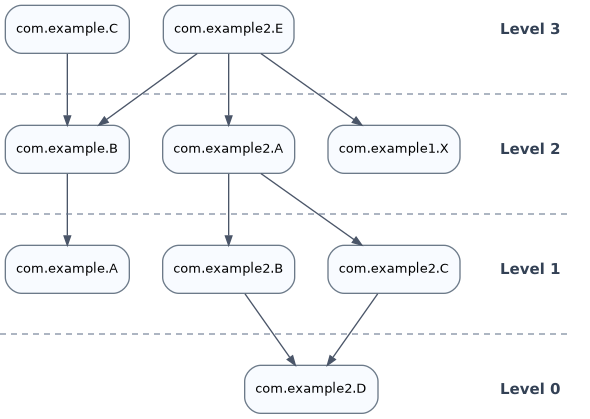
\includegraphics[width=0.75\textwidth]{figures/test-example-classgraph-acyclic-levels.png}
  \caption{Exemplo ac\'iclico de \texttt{test-example-1.0.0.jar}.}
  \label{fig:acyclic-levels}
\end{figure}

As setas entre as caixas s\~ao depend\^encias entre classes por chamada ou uso.
No exemplo, \texttt{com.example.B} usa a classe \texttt{com.example.A}, de
forma abreviada $B \to A$. As linhas horizontais foram acrescentadas
manualmente e visualizam os n\'iveis da camada. O Level~0 forma a base;
n\'iveis mais altos representam elementos que dependem de elementos abaixo
deles.

Esse tipo de representa\c{c}\~ao \'e \'util e amplamente usado. Como
visualiza\c{c}\~ao de aplica\c{c}\~oes reais, por\'em, ele tem tr\^es
problemas pr\'aticos:

\begin{enumerate}
  \item Muitas setas tornam o grafo confuso j\'a em aplica\c{c}\~oes de porte
        m\'edio.
  \item A estrutura de pacotes fica distribu\'ida por v\'arios n\'iveis e n\~ao
        forma um agrupamento vis\'ivel.
  \item Em depend\^encias c\'iclicas, o ciclo precisa ser quebrado para o
        c\'alculo dos n\'iveis, para que surja alguma ordem vertical. O grafo
        original de depend\^encias permanece inalterado; muda apenas o DAG
        derivado (\emph{Directed Acyclic Graph}, um grafo dirigido sem ciclos)
        sobre o qual os n\'iveis s\~ao calculados. A quest\~ao decisiva,
        portanto, \'e qual aresta fica fora desse c\'alculo, pois exatamente
        essa aresta aparece depois como quebra da ordem calculada.
\end{enumerate}

\section{S202 como Representa\c{c}\~ao Hier\'arquica em Camadas}

Com a ferramenta open source S202, buscamos tratar esses problemas de forma
direta. S202 n\~ao substitui simplesmente o grafo plano de classes por uma
representa\c{c}\~ao melhorada. Ele o substitui por uma hip\'otese arquitetural
hier\'arquica: pacotes permanecem vis\'iveis como cont\^eineres e, dentro de
cada cont\^einer, pacotes ou classes s\~ao ordenados de acordo com suas
depend\^encias.

As setas podem ser exibidas opcionalmente. Normalmente, por\'em, a ordem
vertical j\'a deve deixar compreens\'ivel quais partes da aplica\c{c}\~ao
ficam mais acima e quais servem de base. Depend\^encias indesejadas, assim,
n\~ao aparecem apenas como uma linha isolada em uma grande rede, mas como uma
quebra em uma ordem esperada de camadas.

Ao contr\'ario do grafo plano de classes, em S202 os n\'iveis s\~ao
estruturados hierarquicamente pela estrutura de pacotes. Cada pacote ordena
seus filhos diretos, isto \'e, subpacotes ou classes, segundo suas
depend\^encias locais. A estrutura de pacotes permanece vis\'ivel, em vez de
ser espalhada pelo grafo de classes.

\begin{figure}[H]
  \centering
  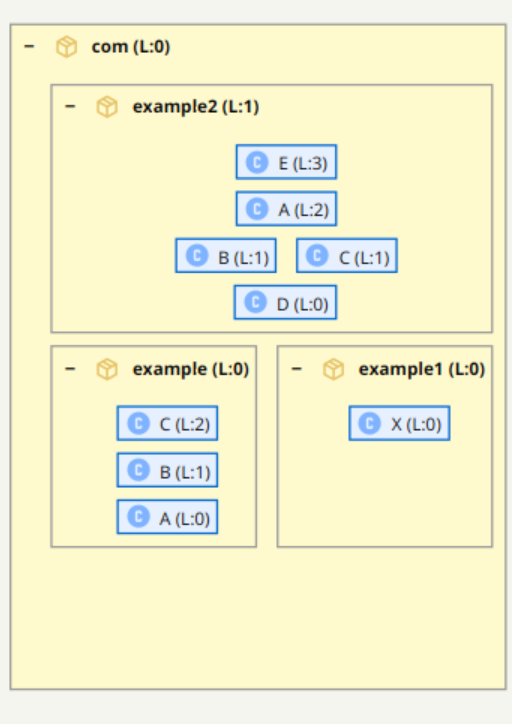
\includegraphics[width=0.55\textwidth]{figures/s202-dependencies-acyclic.png}
  \caption{Representa\c{c}\~ao S202 do exemplo ac\'iclico: pacotes permanecem
  vis\'iveis como cont\^eineres, classes s\~ao ordenadas dentro de seu
  cont\^einer e setas podem ser exibidas quando necess\'ario.}
  \label{fig:s202-acyclic}
\end{figure}

O exemplo mostra a estrutura de pacotes abaixo do pacote externo
\texttt{com}: \texttt{example}, \texttt{example1} e \texttt{example2} s\~ao
sub\'arvores desse cont\^einer. Na sub\'arvore \texttt{example2} existe uma
estrutura interna de classes n\~ao trivial; ao mesmo tempo, a estrutura mais
ampla mostra que \texttt{example2} depende de \texttt{example} e
\texttt{example1}. No n\'ivel de classes vale, para \texttt{example2},
$E \to A \to (B \mid C) \to D$. A representa\c{c}\~ao abstrai
deliberadamente das arestas individuais. Se \texttt{A} tem uma depend\^encia
para \texttt{B}, para \texttt{C} ou para ambos \'e menos importante para a
vis\~ao arquitetural ampla do que a estrutura em camadas do pacote. Exatamente
essa abstra\c{c}\~ao torna redes extensas de rela\c{c}\~oes ainda leg\'iveis.

A ideia n\~ao \'e nova. O produto comercial Structure101 j\'a tinha uma
representa\c{c}\~ao muito semelhante. No entanto, n\~ao h\'a uma
implementa\c{c}\~ao aberta nem uma documenta\c{c}\~ao t\'ecnica que explique
como calcular esse layout de forma confi\'avel. S202 fecha essa lacuna como
ferramenta open source sob a licen\c{c}a Apache.

Este documento descreve as armadilhas t\'ipicas na realiza\c{c}\~ao de um
layout desse tipo e mostra uma solu\c{c}\~ao com a qual muitos desses
problemas podem ser eliminados de forma conceitualmente limpa.

\section{Erros T\'ipicos no C\'alculo de Camadas}

As Figuras~\ref{fig:acyclic-levels} e~\ref{fig:s202-acyclic} mostram
deliberadamente um exemplo simples e ac\'iclico. Nesse caso, a camada \'e
inequ\'ivoca: \texttt{E} fica acima de \texttt{A}, \texttt{A} fica acima de
\texttt{B} e \texttt{C}, e ambos ficam acima de \texttt{D}. N\~ao h\'a
realimenta\c{c}\~ao, portanto nenhuma aresta precisa ser escolhida para ser
ignorada no c\'alculo dos n\'iveis.

Em aplica\c{c}\~oes reais esse caso \'e mais exce\c{c}\~ao do que regra. Assim
que classes ou pacotes dependem ciclicamente uns dos outros, uma passagem
normal pelo grafo n\~ao basta mais. \'E exatamente a\'i que come\c{c}am os
erros interessantes: a representa\c{c}\~ao muitas vezes ainda parece
plaus\'ivel, mas os n\'iveis calculados deixam de ser est\'aveis ou deixam de
ser explic\'aveis em termos arquiteturais.

Nas se\c{c}\~oes seguintes, o termo SCC tem papel central. Uma SCC
(\emph{Strongly Connected Component}, componente fortemente conexa) \'e um
conjunto de n\'os no qual cada n\'o pode alcan\c{c}ar todos os outros por
caminhos dirigidos de depend\^encia. Em um ciclo desse tipo, nem todas as
depend\^encias podem correr para baixo ao mesmo tempo.

Um layout em camadas correto precisa, portanto, satisfazer v\'arios requisitos
ao mesmo tempo:

\begin{enumerate}
  \item Se $A \to B$, ent\~ao $A$ deve ficar acima de $B$.
  \item Pacotes precisam permanecer vis\'iveis como cont\^eineres. Um pacote
        n\~ao deve ser deslocado por acaso apenas porque uma classe contida
        nele tem um n\'ivel de classe alto.
  \item Classes ou pacotes que formam uma SCC precisam ser tratados
        explicitamente, porque em um ciclo nem todas as arestas podem correr
        para baixo ao mesmo tempo.
\end{enumerate}

Esses requisitos s\~ao individualmente bem resolv\'iveis. Juntos, por\'em,
eles criam um sistema circular de depend\^encias entre os pr\'oprios n\'iveis
da computa\c{c}\~ao: n\'iveis de classes influenciam posi\c{c}\~oes
vis\'iveis, cont\^eineres de pacotes estruturam essas posi\c{c}\~oes, e SCCs
for\c{c}am corre\c{c}\~oes em uma ordem que j\'a teria sido calculada sem o
tratamento de ciclos. \'E da\'i que surgem os modos t\'ipicos de falha.

\subsection{Corre\c{c}\~ao Retroativa}

Corre\c{c}\~ao retroativa significa aqui: uma estrutura reconhecida mais tarde
obriga uma altera\c{c}\~ao posterior em n\'iveis j\'a calculados.

Um algoritmo ing\^enuo percorre as classes e atribui n\'iveis diretamente. Ele
v\^e primeiro a classe \texttt{A}, define seu n\'ivel e com isso tamb\'em
eleva o pacote de \texttt{A}. Mais tarde encontra a classe \texttt{B} e
reconhece: \texttt{A} e \texttt{B} pertencem \`a mesma SCC e precisam ser
tratadas em conjunto. Agora \texttt{A} teria de ser corrigida, e com ela seu
pacote e possivelmente outros pacotes que dependem dele.

O problema n\~ao \'e a corre\c{c}\~ao em si. O problema \'e que partes do
layout, nesse momento, j\'a foram tratadas como conclu\'idas. Um algoritmo que
mistura detec\c{c}\~ao de ciclos e atribui\c{c}\~ao de n\'iveis precisa
alterar retroativamente lugares que ele na verdade j\'a deixou para tr\'as.

\subsection{Resultados Dependentes da Ordem}

Classes v\^em de JARs. A ordem em que uma ferramenta v\^e classes n\~ao segue
a arquitetura, mas a ordem de empacotamento do JAR, a ordem dos m\'odulos, a
ferramenta de build ou detalhes do sistema de arquivos. Se um algoritmo trata
ciclos incidentalmente durante essa travessia, o resultado depende dessa ordem
acidental.

Isso \'e perigoso porque o erro n\~ao precisa ser vis\'ivel imediatamente. O
grafo ainda pode parecer aproximadamente correto. Mesmo assim, a mesma base de
c\'odigo pode receber n\'iveis diferentes dependendo da configura\c{c}\~ao de
build.

\subsection{Mistura de N\'iveis de Classe e de Pacote}

Um erro natural \'e derivar o n\'ivel de um pacote a partir do maior n\'ivel de
suas classes contidas. Isso parece plaus\'ivel, mas mistura duas perguntas
diferentes: onde uma classe fica no grafo de classes e onde um pacote fica na
hip\'otese arquitetural.

Um pacote n\~ao est\'a arquiteturalmente alto apenas porque por acaso cont\'em
uma classe posicionada alto. A regra central \'e:

\begin{quote}
  N\'iveis de pacotes surgem de depend\^encias entre pacotes, n\~ao da altura
  m\'axima de classes individuais.
\end{quote}

Isso parece trivial, mas n\~ao \'e. Justamente porque pacotes s\~ao
cont\^eineres de classes, parece natural derivar sua posi\c{c}\~ao das classes
contidas. Mas \'e exatamente assim que se misturam dois n\'iveis que precisam
permanecer separados. Somente quando n\'iveis de pacotes surgem de
depend\^encias entre pacotes, os pacotes permanecem unidades arquiteturais
est\'aveis. Caso contr\'ario, uma \'unica classe fora do padr\~ao basta para
elevar o pacote ao n\'ivel errado e tornar inutiliz\'avel o cont\^einer que
deveria oferecer orienta\c{c}\~ao.

A mesma mistura existe um n\'ivel acima. Se o n\'ivel de um pacote for
calculado a partir de um grafo que tamb\'em carrega as depend\^encias entre
seus pr\'oprios subpacotes, um pacote sobe apenas porque \'e profundamente
estratificado por dentro. Um pacote que cont\'em tudo o que usa pertence ao
n\'ivel~0, independentemente de como seus filhos se relacionam entre si. A
regra completa diz, portanto: o n\'ivel de um elemento surge apenas de
depend\^encias que saem do seu pr\'oprio interior.

\subsection{O Grande Lago}

A resposta formalmente limpa para ciclos \'e: todos os elementos de uma SCC
recebem o mesmo n\'ivel. Para ciclos pequenos isso \'e aceit\'avel. Em sistemas
reais, por\'em, SCCs podem ficar muito grandes. Ent\~ao centenas ou milhares
de classes acabam no mesmo n\'ivel. A camada desaparece; o que resta \'e um
bloco plano.

O ciclo, assim, foi reconhecido corretamente, mas deixou de ser visualizado de
forma \'util. Uma ferramenta precisa, portanto, conseguir quebrar SCCs grandes.
O ponto decisivo \'e que as arestas cortadas n\~ao podem desaparecer. Elas
precisam permanecer vis\'iveis, porque explicam por que a ordem calculada vale
apenas como hip\'otese arquitetural.

\section{Dois Tipos de Ciclos}

S202 distingue dois tipos fundamentalmente diferentes de ciclos e torna ambos
vis\'iveis como overlays ativados separadamente:

\begin{description}
  \item[Ciclos de classes (roxo)] Componentes fortemente conexas no n\'ivel
        de classes. Duas ou mais classes que dependem uma da outra direta ou
        transitivamente formam tal ciclo. Ciclos de classes revelam acoplamento
        no n\'ivel de implementa\c{c}\~ao que impede uma ordem linear estrita de
        classes individuais. Eles s\~ao detectados pelo algoritmo de Tarjan sobre
        o grafo de depend\^encias de classes.
  \item[Ciclos de pacotes (laranja)] Tangles dentro de um cont\^einer. Um
        cont\^einer \'e um pacote (ou a raiz); seus filhos s\~ao as classes e
        os subpacotes que ele cont\'em diretamente. Dois filhos dependem um do
        outro assim que qualquer classe na sub\'arvore de um usa uma classe na
        sub\'arvore do outro. Quando filhos de um cont\^einer formam um ciclo
        dessa maneira e pelo menos um deles \'e um pacote, h\'a um ciclo de
        pacotes, independentemente de quais classes concretas s\~ao
        respons\'aveis. Ciclos de pacotes revelam acoplamento no n\'ivel
        arquitetural: a pr\'opria estrutura de pacotes tem depend\^encias
        circulares. Um ciclo formado apenas por classes do mesmo pacote n\~ao
        \'e um ciclo de pacotes; o overlay roxo o mostra.
\end{description}

A distin\c{c}\~ao importa porque os dois tipos respondem a perguntas diferentes:

\begin{itemize}
  \item Um \emph{ciclo de classes} mostra quais classes concretas precisam ser
        desembaraladas. Dissolv\^e-lo frequentemente exige mover um m\'etodo,
        extrair uma interface ou inverter uma depend\^encia entre duas classes
        espec\'ificas.
  \item Um \emph{ciclo de pacotes} mostra onde os pr\'oprios limites de pacotes
        est\~ao quebrados. Resolv\^e-lo pode exigir uma reestrutura\c{c}\~ao
        maior~-- como mesclar dois pacotes, introduzir um novo, ou redefinir
        inteiramente a divis\~ao de m\'odulos.
\end{itemize}

Um ciclo de pacotes pode existir mesmo quando nenhum ciclo de classes individual
\'e vis\'ivel~-- por exemplo, quando dois pacotes se chamam mutuamente por meio
de classes diferentes que s\~ao individualmente ac\'iclicas. Por outro lado, um
ciclo de classes inteiramente contido em um \'unico pacote n\~ao implica
necessariamente um ciclo de pacotes.

Como os dois overlays respondem a perguntas diferentes, S202 os mant\'em como
chaves independentes. Ativar ambos ao mesmo tempo \'e poss\'ivel e \'util ao
buscar a causa raiz de um problema arquitetural, mas cada overlay tamb\'em \'e
significativo por si s\'o: o overlay de ciclos de pacotes revela a forma
estrutural do problema, enquanto o overlay de ciclos de classes revela as
arestas concretas que o causam.

\section{O Cont\^einer como Unidade de Ordena\c{c}\~ao}

A solu\c{c}\~ao escolhida por S202 consiste em separar consistentemente
an\'alise, ordena\c{c}\~ao e representa\c{c}\~ao. O grafo de classes permanece
o modelo bruto das depend\^encias reais. Ele n\~ao \'e alterado s\'o porque uma
representa\c{c}\~ao em camadas precisa de um DAG. Em vez disso, S202 deriva
desse grafo vistas adicionais: SCCs para a detec\c{c}\~ao de ciclos, um grafo
ponderado de irm\~aos por cont\^einer para a ordena\c{c}\~ao e uma estrutura
hier\'arquica de interface para a representa\c{c}\~ao.

Hip\'otese arquitetural n\~ao significa aqui uma arquitetura-alvo afirmada.
Significa uma arquitetura real derivada das depend\^encias observadas: a ordem
que corresponde mais estreitamente ao c\'odigo existente e \`as suas
depend\^encias, sem esconder onde essa ordem \'e quebrada por ciclos ou back
edges.

A unidade de ordena\c{c}\~ao \'e o cont\^einer. Cada pacote ordena seus filhos
diretos~-- classes e subpacotes igualmente~-- exclusivamente pelas
depend\^encias que correm entre esses filhos. O que acontece dentro de um filho
\'e assunto desse filho; o que sai do cont\^einer \'e assunto do seu pacote pai.
Structure101 constr\'oi seus \emph{Levelized Structure Maps} pela mesma regra.
Ela \'e o passo decisivo: uma depend\^encia entre classes \'e contada
exatamente uma vez, a saber, no cont\^einer que cont\'em ambas as pontas como
filhos de sub\'arvores diferentes. N\~ao h\'a ordem global de pacotes da qual a
ordem local seria derivada e, portanto, tamb\'em n\~ao h\'a ordem local que
possa contradizer uma global. Um pacote permanece est\'avel como cont\^einer
porque apenas suas rela\c{c}\~oes com seus irm\~aos determinam sua posi\c{c}\~ao.
Ao mesmo tempo, a ordem do cont\^einer fornece um crit\'erio para n\~ao
escolher back edges arbitrariamente, mas marc\'a-los como viola\c{c}\~oes
concretas da ordem esperada.

Com isso, os modos de erro descritos acima desaparecem n\~ao por um \'unico
truque algor\'itmico, mas por uma responsabilidade clara: cada cont\^einer
decide por si e de forma definitiva. Primeiro as depend\^encias s\~ao
analisadas, depois determina-se por cont\^einer uma ordem plaus\'ivel, em
seguida constr\'oi-se a estrutura vis\'ivel e, por fim, verifica-se se a
representa\c{c}\~ao cumpre sua pr\'opria afirma\c{c}\~ao.

\section{De Depend\^encias de Classes \`a Ordem dos Cont\^eineres}

Em S202, o grafo plano de classes n\~ao \'e o modelo de layout vis\'ivel. Ele
\'e um artefato de an\'alise: serve para capturar depend\^encias concretas,
detectar SCCs e atribuir cada depend\^encia ao cont\^einer que decide sua
dire\c{c}\~ao. A figura vis\'ivel de S202 surge depois a partir da estrutura
de pacotes e da ordem dentro de cada cont\^einer.

Uma depend\^encia entre classes surge de uma chamada ou refer\^encia de m\'etodo,
de uma instancia\c{c}\~ao, de heran\c{c}a ou de uma refer\^encia pura de tipo:
tipo de campo, de par\^ametro ou de retorno, argumento de tipo, cast,
anota\c{c}\~ao ou exce\c{c}\~ao capturada. Todas contam igualmente, pois em
nenhum desses casos o c\'odigo compila sem a outra classe. Quanto custa remover a
depend\^encia \'e uma quest\~ao \`a parte, respondida pelo peso. Classes
aninhadas, locais e an\^onimas n\~ao s\~ao n\'os pr\'oprios: aquilo de que elas
dependem e aquilo que depende delas conta para a classe que as envolve.

Para cada depend\^encia entre classes $X \to Y$, S202 determina o cont\^einer
mais profundo que cont\'em $X$ e $Y$ e os dois filhos desse cont\^einer em
cujas sub\'arvores $X$ e $Y$ se encontram. A depend\^encia torna-se uma aresta
entre esses dois irm\~aos~-- e somente a\'i:

\begin{lstlisting}
com.a.X -> com.b.c.Y    conteiner com     aresta com.a   -> com.b
com.a.X -> com.a.Y      conteiner com.a   aresta com.a.X -> com.a.Y
com.a.X -> com.a.b.Y    conteiner com.a   aresta com.a.X -> com.a.b
\end{lstlisting}

O peso de uma aresta entre irm\~aos \'e a soma das chamadas de m\'etodo de
todas as depend\^encias entre classes projetadas sobre ela; uma depend\^encia
sem chamadas~-- heran\c{c}a ou uma refer\^encia pura de tipo~-- contribui com um
peso de fallback de~1. Nada \'e
propagado: nem o lado de origem nem o de destino \'e multiplicado ao longo da
cadeia de ancestrais. O n\'umero de arestas \'e limitado pelo n\'umero de
depend\^encias entre classes, e cada depend\^encia tem exatamente um lugar em
que sua dire\c{c}\~ao \'e decidida. Classes e pacotes s\~ao n\'os iguais nesse
grafo; uma classe diretamente no pacote e um subpacote do mesmo pacote s\~ao
ordenados um contra o outro.

Ciclos em um grafo de irm\~aos s\~ao os tangles desse cont\^einer. Antes do
c\'alculo dos n\'iveis, o grafo precisa ser ac\'iclico. Quando irm\~aos
formam uma SCC, S202 usa uma medida de rank para avaliar se um irm\~ao tende a
usar os outros ou a ser usado por eles:

\[
  rank(S) = \frac{out(S) - in(S)}{\max(1,\; out(S) + in(S))}
\]

$out(S)$ \'e a soma dos pesos das arestas de $S$ para outros membros da mesma
SCC, $in(S)$ a soma dos pesos das arestas desses membros para $S$. Um rank
positivo significa: o elemento usa mais do que \'e usado; tende a pertencer ao
topo. Um rank negativo significa: o elemento \'e mais usado e tende a
pertencer \`a base.

Dentro de uma SCC, todas as arestas $S \to T$ com $rank(S) < rank(T)$ s\~ao
cortadas~-- ou seja, todas as arestas que correm contra o fluxo de
depend\^encias. N\~ao se usa limiar: qualquer diferen\c{c}a mensur\'avel de rank
basta como justificativa para um corte. Se todos os ranks dentro de uma SCC
forem iguais, a topologia n\~ao fornece informa\c{c}\~ao de dire\c{c}\~ao. Nesse
caso, todas as arestas internas s\~ao removidas e os n\'iveis dos n\'os
afetados surgem exclusivamente de depend\^encias fora da antiga SCC. Se
tamb\'em n\~ao houver depend\^encias a\'i, os n\'os permanecem no mesmo
n\'ivel~-- como verdadeiros pares sem ordem justific\'avel.

Ambos os tipos de corte s\~ao aplicados iterativamente: ap\'os cada passagem,
as SCCs s\~ao recalculadas e, para SCCs residuais, os ranks s\~ao recalculados
sobre seus membros. O procedimento termina quando n\~ao resta nenhuma SCC com
pelo menos dois membros. A detec\c{c}\~ao de simetria baseia-se na medida de
rank, n\~ao em uma compara\c{c}\~ao de pesos: uma SCC em que todas as arestas
t\^em o mesmo peso n\~ao \'e necessariamente sim\'etrica, porque graus de
entrada e sa\'ida diferentes produzem ranks diferentes apesar de pesos iguais.
As arestas entre irm\~aos cortadas s\~ao os \emph{back edges de cont\^einer}.
Structure101 procura neste ponto um conjunto t\~ao pequeno quanto poss\'ivel
de arestas de realimenta\c{c}\~ao; o corte por rank \'e um substituto
determin\'istico sem pretens\~ao de minimalidade. Ele \'e independente da
ordem porque todos os elementos s\~ao processados em ordem classificada.

Ap\'os esse tratamento de ciclos, S202 calcula os n\'iveis no DAG resultante.
O n\'ivel~0 \'e formado pelos irm\~aos que n\~ao usam nenhum outro irm\~ao.
Cada outro irm\~ao fica um n\'ivel acima do irm\~ao mais alto que usa
diretamente. Assim surge a estratifica\c{c}\~ao transitiva: de $B \to A$ e
$C \to B$ segue $A$ no n\'ivel~0, $B$ no n\'ivel~1 e $C$ no n\'ivel~2, mesmo
que n\~ao exista aresta direta $C \to A$.

Essa regra~-- conhecida como \emph{longest-path} ou \emph{leveliza\c{c}\~ao
ASAP}~-- ancora cada elemento o mais baixo poss\'ivel, imediatamente acima da
sua depend\^encia mais profunda. Ela coincide com a invariante que Structure101
documenta para seus Levelized Structure Maps: cada elemento depende de pelo
menos um elemento no n\'ivel imediatamente abaixo. A alternativa de puxar cada
elemento rente \emph{abaixo do seu consumidor} (ALAP) violaria essa
invariante, pois poderia abrir-se uma lacuna entre um elemento e sua
depend\^encia mais pr\'oxima.

Uma consequ\^encia \'e aceita deliberadamente: irm\~aos com o mesmo papel, mas
cadeias de depend\^encia de profundidades diferentes, acabam em n\'iveis
diferentes. Se v\'arios adaptadores ficam acima da mesma camada de
aplica\c{c}\~ao, mas um deles fica adicionalmente acima de um pacote utilit\'ario
compartilhado, esse um fica um n\'ivel acima dos demais~-- a leveliza\c{c}\~ao
mede profundidade de depend\^encia, n\~ao papel arquitetural.

O \emph{localLevel} assim calculado \'e a hip\'otese arquitetural. Ele
determina a posi\c{c}\~ao de cada elemento dentro do seu cont\^einer, e a
cadeia de localLevels da raiz at\'e o elemento \'e a ordem contra a qual as
viola\c{c}\~oes s\~ao medidas. Ele \'e deliberadamente local: compara apenas
irm\~aos.

Al\'em disso, S202 mant\'em para cada elemento um \emph{architectureLevel}
global. Ele mede qu\~ao profunda \'e, de fato, a cadeia de depend\^encias abaixo
de um elemento e \'e, portanto, uma medida da sua complexidade; a altura padr\~ao
na vista 3D (onde qualquer outra m\'etrica pode ser escolhida) e o anel da
vista hexagonal baseiam-se nele. O
\emph{architectureLevel} de uma classe \'e sua profundidade longest-path no
grafo de classes. S\~ao deixados de fora apenas os \emph{cortes de n\'ivel}:
back edges que est\~ao dentro de um ciclo de classes. Um back edge que apenas
corre contra a ordem de dois pacotes, sem fechar um ciclo de classes, \'e uma
depend\^encia ac\'iclica real e continua contando. O \emph{architectureLevel}
de um pacote segue a mesma regra um n\'ivel acima: \'e sua profundidade
longest-path em um grafo de pacotes em que $P$ depende de $Q$ sempre que um
n\~ao-back-edge leva da sub\'arvore de $P$ para a sub\'arvore de $Q$ e nenhum
dos dois pacotes cont\'em o outro. Ambos os grafos s\~ao ac\'iclicos por
constru\c{c}\~ao. Um pacote nunca \'e, assim, elevado pelo seu pr\'oprio
interior: quem cont\'em tudo o que usa fica no n\'ivel~0. O n\'ivel global n\~ao
influencia nem o layout nem a detec\c{c}\~ao de viola\c{c}\~oes.

\section{Do Ciclo de Classes ao Back Edge}

A Figura~\ref{fig:cyclic-class} mostra um exemplo c\'iclico do Example JAR
como grafo cl\'assico de classes. Os dois subgrafos para Notification e
Payment cont\^em realimenta\c{c}\~oes.

\begin{figure}[H]
  \centering
  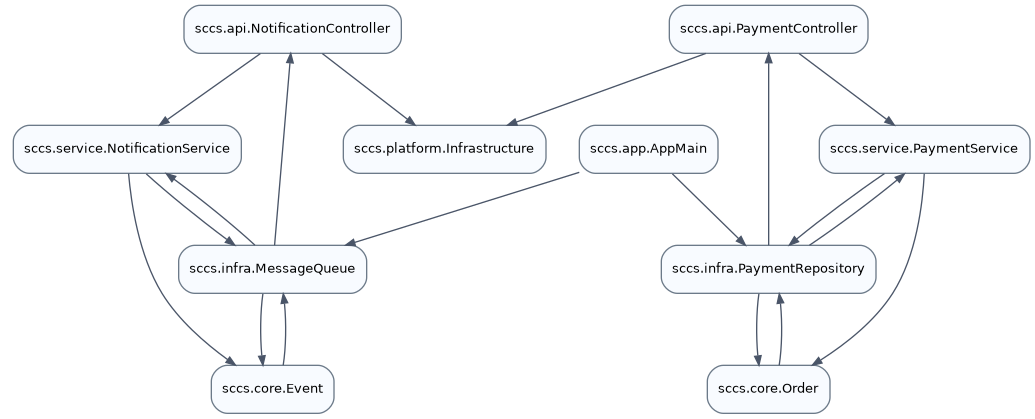
\includegraphics[width=0.9\textwidth]{figures/test-example-classgraph-cyclic.png}
  \caption{Exemplo c\'iclico de \texttt{test-example-1.0.0.jar}. Em cada ciclo,
  pelo menos uma aresta precisa ser cortada para o c\'alculo dos n\'iveis.}
  \label{fig:cyclic-class}
\end{figure}

As regi\~oes c\'iclicas marcadas s\~ao duas SCCs n\~ao triviais: uma SCC de
Notification com \texttt{NotificationController},
\texttt{NotificationService}, \texttt{MessageQueue} e \texttt{Event}, e uma
SCC de Payment com \texttt{PaymentController}, \texttt{PaymentService},
\texttt{PaymentRepository} e \texttt{Order}. O procedimento estabelecido para
encontrar esses componentes \'e o algoritmo de Tarjan.

No caso c\'iclico, o grafo de classes coloca a pergunta t\'ecnica: qual aresta
precisa ser ignorada para que a SCC volte a ser um DAG calcul\'avel para a
atribui\c{c}\~ao de n\'iveis? O grafo de classes sozinho n\~ao fornece um
crit\'erio arquitetural para isso. A ordem do cont\^einer o fornece: uma
depend\^encia entre classes \'e um back edge exatamente quando sua proje\c{c}\~ao
no seu cont\^einer \'e uma aresta entre irm\~aos cortada.

Um ciclo de classes que est\'a dentro de um pacote \'e cortado dentro desse
pacote~-- a\'i as pr\'oprias classes s\~ao os irm\~aos. Um ciclo de classes que
atravessa v\'arios pacotes aparece no cont\^einer pai comum como tangle entre
pacotes e \'e cortado a\'i; dentro dos pacotes envolvidos, contam apenas as
arestas cujas duas pontas est\~ao dentro deles. A corre\c{c}\~ao retroativa do
cat\'alogo de erros n\~ao pode surgir desse modo: nenhum cont\^einer precisa
rever uma decis\~ao de outro.

Disso segue uma propriedade que pode ser provada: todo ciclo de classes
cont\'em pelo menos um back edge. No cont\^einer mais profundo que cont\'em
todas as classes do ciclo, ele se projeta sobre um ciclo entre irm\~aos, e a\'i
pelo menos uma aresta foi cortada. Para o n\'ivel global das classes basta,
portanto, deixar de fora os back edges dentro de ciclos de classes~-- os
\emph{cortes de n\'ivel}. O grafo de classes fica ent\~ao ac\'iclico; o
c\'alculo dos n\'iveis n\~ao precisa de nenhum tratamento adicional de ciclos
nem de casos especiais.

Os back edges fora de ciclos de classes, por outro lado, permanecem no
c\'alculo dos n\'iveis. Dois pacotes podem usar um ao outro por meio de classes
diferentes sem que surja um ciclo de classes. A aresta contra a ordem dos
pacotes \'e ent\~ao uma viola\c{c}\~ao na imagem, mas continua fazendo parte da
profundidade real de depend\^encia da sua classe.

Todos os back edges s\~ao registrados como achados \emph{classBackEdge} e
permanecem vis\'iveis como arestas de viola\c{c}\~ao vermelhas.

\begin{figure}[H]
  \centering
  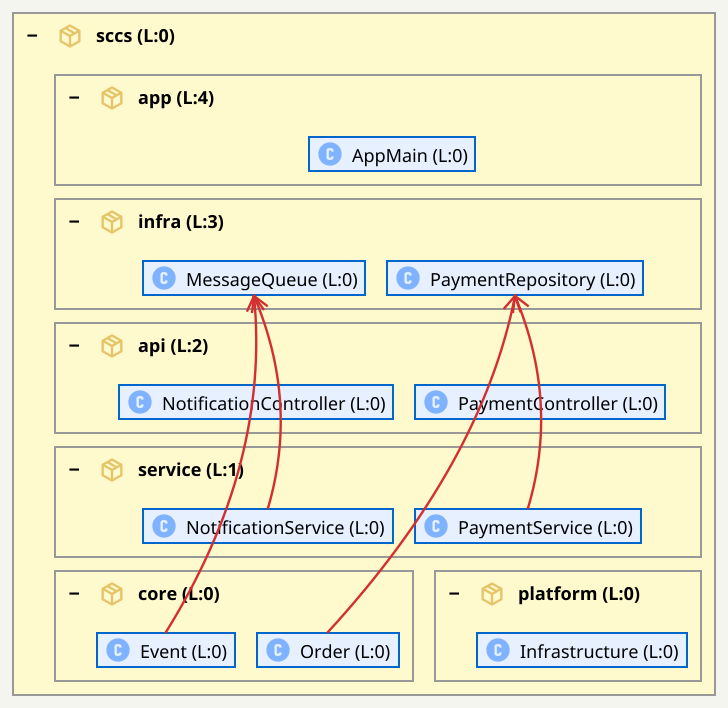
\includegraphics[width=0.6\textwidth]{figures/s202-dependencies-cyclic.png}
  \caption{Exemplo c\'iclico na representa\c{c}\~ao de S202. As arestas
  vermelhas s\~ao viola\c{c}\~oes: correm contra a ordem de cont\^einer calculada
  e permanecem como achado vis\'ivel da hip\'otese arquitetural. Todas as quatro
  arestas vermelhas s\~ao back edges: proje\c{c}\~oes das arestas entre irm\~aos
  \texttt{core}$\to$\texttt{infra} e \texttt{service}$\to$\texttt{infra},
  cortadas no cont\^einer \texttt{sccs}.}
  \label{fig:s202-cyclic}
\end{figure}

Os termos back edge e viola\c{c}\~ao descrevem pap\'eis diferentes das mesmas
arestas:

\begin{description}
  \item[Back edge] Uma depend\^encia entre classes cuja proje\c{c}\~ao no seu
        cont\^einer foi cortada ao quebrar um tangle. Pertence ao tratamento
        de ciclos. Se al\'em disso estiver dentro de um ciclo de classes, \'e
        um corte de n\'ivel e \'e deixada de fora do n\'ivel global das classes.
  \item[Viola\c{c}\~ao] Uma depend\^encia concreta que corre para cima na ordem
        calculada. O que conta aqui \'e a ordem \emph{aninhada}, n\~ao um n\'ivel
        global plano: as cadeias de \emph{localLevel} das duas pontas s\~ao
        comparadas a partir do cont\^einer comum mais externo para baixo, entrada
        por entrada, e a dire\c{c}\~ao \'e decidida pela primeira entrada em que
        os dois n\'iveis diferem (chamado \emph{visual rank} no c\'odigo); se uma
        cadeia termina antes de tal entrada, nenhuma das pontas fica acima da
        outra. Toda viola\c{c}\~ao \'e um back
        edge, porque fora das arestas cortadas todas as arestas entre irm\~aos
        correm para baixo. Inversamente, um back edge corre para cima ou para o
        lado; s\'o quando um segundo caminho dentro de um tangle j\'a fixa a
        dire\c{c}\~ao \'e que uma aresta cortada pode acabar apontando para baixo,
        e ent\~ao n\~ao \'e uma viola\c{c}\~ao vis\'ivel. Conceitualmente, uma
        viola\c{c}\~ao continua sendo o desvio vis\'ivel da ordem, enquanto um
        back edge descreve o papel da aresta no tratamento de ciclos.
\end{description}

S202, portanto, n\~ao esconde o ciclo. Arestas classificadas como back edges
permanecem vis\'iveis como viola\c{c}\~oes porque explicam por que a ordem do
cont\^einer n\~ao corresponde completamente \`as depend\^encias concretas entre
classes. Com isso, o desvio torna-se rastre\'avel em vez de arbitr\'ario.

\section{Verifica\c{c}\~ao Redundante da Consist\^encia}

As etapas descritas at\'e aqui j\'a mostram por que a implementa\c{c}\~ao \'e
propensa a erros. N\~ao basta proteger algoritmos isolados com unit tests.
Muitos erros surgem apenas da intera\c{c}\~ao dos dados: depend\^encias
concretas entre classes, estrutura de pacotes, SCCs, pesos agregados de
pacotes e posi\c{c}\~oes locais de representa\c{c}\~ao influenciam-se
mutuamente.

Por isso S202 n\~ao verifica apenas passos individuais de c\'alculo. Depois
que toda a pipeline rodou, o resultado final \'e verificado de forma
redundante contra regras de consist\^encia. Essas regras n\~ao recalculam o
layout e n\~ao corrigem nada. Elas apenas leem o resultado e perguntam: a
representa\c{c}\~ao gerada \'e consistente em si mesma?

A verifica\c{c}\~ao consiste em cinco regras:

\begin{enumerate}
  \item \textbf{Grafo de classes:} Para cada depend\^encia entre classes
        $A \to B$ que n\~ao \'e um corte de n\'ivel, $A$ est\'a em um n\'ivel
        mais alto que $B$, e todo corte de n\'ivel \'e um back edge. N\~ao h\'a
        outras exce\c{c}\~oes, porque o grafo de classes sem cortes de n\'ivel
        \'e ac\'iclico.
  \item \textbf{Cont\^einer:} Em cada cont\^einer, cada aresta entre irm\~aos
        que n\~ao foi cortada corre de um \emph{localLevel} mais alto para um
        mais baixo. Essa \'e a promessa da pr\'opria representa\c{c}\~ao.
  \item \textbf{Back edges s\'o em tangles:} Cada aresta entre irm\~aos cortada
        liga dois membros do mesmo tangle de cont\^einer. Nada \'e cortado fora
        de ciclos.
  \item \textbf{Grafo de pacotes:} Para cada n\~ao-back-edge entre classes de
        dois pacotes que n\~ao se cont\^em mutuamente, o pacote de origem fica
        acima do pacote de destino.
  \item \textbf{Representa\c{c}\~ao vis\'ivel:} Toda depend\^encia que corre para
        cima na ordem aninhada \'e um back edge. A figura n\~ao mostra nenhuma
        viola\c{c}\~ao que o modelo n\~ao conhe\c{c}a.
\end{enumerate}

Essas regras de consist\^encia n\~ao s\~ao uma otimiza\c{c}\~ao adicional nem
um segundo algoritmo de layout. Elas s\~ao uma verifica\c{c}\~ao independente
de plausibilidade ap\'os o fim do c\'alculo. Exatamente por isso encontram
erros que faltam facilmente em unit tests normais: uma aresta foi cortada
silenciosamente no layout sem contar como back edge; um back edge est\'a fora
de qualquer tangle; uma aresta normal corre para cima. Exatamente o primeiro
desses erros passou despercebido por muito tempo em uma vers\~ao anterior de
S202, porque a ordem vinha de um grafo global de pacotes e a posi\c{c}\~ao de um
grafo local de irm\~aos, e ningu\'em verificava se os dois concordavam.

O ponto decisivo \'e a redund\^ancia. A pipeline gera a representa\c{c}\~ao. As
regras verificam em seguida se essa representa\c{c}\~ao cumpre sua pr\'opria
afirma\c{c}\~ao. Com isso, uma simples figura se torna um modelo verific\'avel.

\section{Da Visualiza\c{c}\~ao \`a A\c{c}\~ao}

Uma hip\'otese arquitetural calculada \'e especialmente \'util quando n\~ao
apenas descreve um estado, mas torna mudan\c{c}as planej\'aveis. Para isso,
S202 cont\'em uma an\'alise what-if: classes e pacotes podem ser movidos por
drag and drop na representa\c{c}\~ao. O modelo n\~ao \'e refatorado
imediatamente; em vez disso, a ferramenta calcula quais depend\^encias
passariam a correr para cima na nova disposi\c{c}\~ao.

As viola\c{c}\~oes se atualizam ap\'os cada deslocamento. Assim fica vis\'ivel
se uma reordena\c{c}\~ao planejada torna a arquitetura mais consistente ou
cria novos problemas. Isso \'e importante sobretudo em situa\c{c}\~oes nas
quais a ferramenta n\~ao encontra mais uma ordem inequ\'ivoca: SCCs grandes,
depend\^encias sim\'etricas entre pacotes ou acoplamentos historicamente
crescidos nem sempre podem ser resolvidos automaticamente de maneira sensata.

\begin{figure}[H]
  \centering
  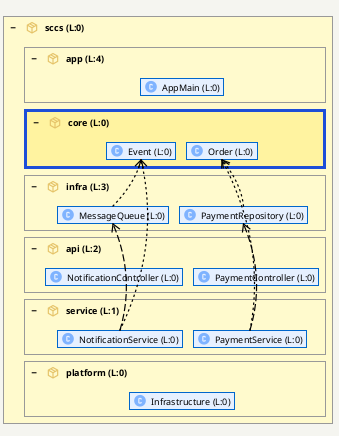
\includegraphics[width=0.45\textwidth]{figures/whatif-core-over-infra.png}
  \caption{Movimento what-if: o pacote \texttt{core} \'e movido do Level~0 para
  entre o Level~3 e o Level~4. Isso cria seis viola\c{c}\~oes, porque
  depend\^encias existentes agora correm contra a disposi\c{c}\~ao escolhida.}
  \label{fig:whatif-core-over-infra}
\end{figure}

A Figura~\ref{fig:whatif-core-over-infra} mostra exatamente essa forma de
trabalho: a disposi\c{c}\~ao manual j\'a n\~ao corresponde \`a ordem calculada
a partir das depend\^encias. Ela pode, mesmo assim, expressar uma
arquitetura-alvo desejada, por exemplo se \texttt{core} deve ficar
conceitualmente acima da infraestrutura. S202, portanto, n\~ao trata essa
decis\~ao como erro da representa\c{c}\~ao, mas torna vis\'ivel seu custo:
nesse caso, seis rela\c{c}\~oes concretas teriam de ser refatoradas ou
desacopladas para que as depend\^encias voltassem a combinar com a camada
escolhida.

Complementarmente, existe uma l\'ogica manual de CUT. Back edges podem ser
marcados de forma direcionada como cortes planejados, e a ferramenta pode em
seguida verificar se esses cortes realmente dissolvem a SCC afetada. O
usu\'ario n\~ao v\^e apenas qual aresta seria uma quebra plaus\'ivel da ordem,
mas tamb\'em pode verificar o efeito desse corte sobre o ciclo.

O que se corta \'e a depend\^encia entre duas classes. Para cada corte, a
ferramenta mostra o que a sustenta: as chamadas de m\'etodo individuais e as
demais refer\^encias~-- campos, par\^ametros, casts~-- que mant\^em a
depend\^encia viva mesmo quando todas as chamadas foram removidas. Um ciclo
muitas vezes surge de poucos pontos concretos do c\'odigo, n\~ao da
rela\c{c}\~ao funcional completa entre duas classes; a ferramenta indica esses
pontos e, com isso, o esfor\c{c}o que um corte representa.

\section{Implementa\c{c}\~ao em N\'ivel Conceitual}

A implementa\c{c}\~ao separa deliberadamente o c\'alculo em v\'arias fases. O
ponto decisivo \'e que nenhuma fase fixa uma posi\c{c}\~ao vis\'ivel antes de
estarem dispon\'iveis as informa\c{c}\~oes que justificam essa posi\c{c}\~ao.

\begin{enumerate}
  \item \textbf{Construir o grafo de classes:} A partir do bytecode \'e gerado
        um grafo dirigido de classes. Esse grafo permanece o modelo bruto da
        an\'alise. Entram no c\'alculo da ordem arestas de todos os tipos:
        \texttt{extends}, \texttt{implements}, \texttt{imports},
        \texttt{instantiates}, \texttt{calls}, heran\c{c}a com uma classe
        aninhada em uma das pontas e refer\^encias puras de tipo
        (\texttt{uses}). Classes aninhadas contam para a classe que as envolve.
  \item \textbf{Detectar SCCs:} No grafo de classes, componentes fortemente
        conexas s\~ao determinadas com Tarjan. O resultado ainda n\~ao \'e um
        layout, mas a informa\c{c}\~ao de quais classes podem ser ordenadas
        aciclicamente e quais pertencem a ciclos (overlay roxo).
  \item \textbf{Ordenar os cont\^eineres:} Cada depend\^encia entre classes \'e
        projetada sobre os dois filhos do cont\^einer comum mais profundo e
        contada a\'i como aresta ponderada entre irm\~aos. Por cont\^einer, as
        SCCs do grafo de irm\~aos s\~ao registradas como tangles (overlay
        laranja), resolvidas com o corte por rank, e a ordem restante \'e
        traduzida por longest-path em um \emph{localLevel} por filho. As
        arestas entre irm\~aos cortadas s\~ao os back edges de cont\^einer.
  \item \textbf{Derivar back edges de classes:} Uma depend\^encia entre classes
        \'e um back edge quando sua proje\c{c}\~ao foi cortada. Ela \'e mantida
        como achado \emph{classBackEdge} e mostrada como aresta de
        viola\c{c}\~ao vermelha.
  \item \textbf{Calcular n\'iveis globais:} O \emph{architectureLevel} de
        classes surge por longest-path no grafo de classes sem os cortes de
        n\'ivel~-- os back edges dentro de ciclos de classes~--, o de pacotes
        no grafo de pacotes de n\~ao-back-edges entre sub\'arvores diferentes.
        Ambos os grafos s\~ao ac\'iclicos por constru\c{c}\~ao.
  \item \textbf{Verificar consist\^encia:} Por fim, a representa\c{c}\~ao final
        \'e verificada de forma redundante contra as cinco regras de
        consist\^encia.
\end{enumerate}

Em resumo:

\begin{lstlisting}
Bytecode -> grafo de classes -> SCCs de classes (overlay roxo)
         -> por conteiner: grafo de irmaos -> tangles (overlay laranja)
                           -> corte por rank (back edges) -> localLevel
         -> back edges de classes -> cortes de nivel
         -> architectureLevel (classes, pacotes)
         -> regras de consistencia
\end{lstlisting}

\section{Conclus\~ao}

S202 calcula, a partir das depend\^encias existentes, a hip\'otese mais
plaus\'ivel da arquitetura real. O resultado \'e uma representa\c{c}\~ao
hier\'arquica em camadas e verific\'avel: depend\^encias entre classes
fornecem o grafo, cada cont\^einer ordena seus filhos exatamente por essas
depend\^encias, back edges tornam vis\'iveis as quebras necess\'arias, e regras
de consist\^encia
verificam se a representa\c{c}\~ao final cumpre sua pr\'opria
afirma\c{c}\~ao.

Uma decis\~ao de projeto fundamental \'e a separa\c{c}\~ao expl\'icita de dois
tipos de ciclos. Ciclos de classes e ciclos de pacotes s\~ao detectados
independentemente, armazenados como achados distintos e expostos por meio de
chaves separadas na interface. Ciclos de classes (roxo) mostram quais classes
concretas formam cadeias c\'iclicas de depend\^encia; ciclos de pacotes (laranja)
mostram quais pacotes s\~ao mutuamente dependentes no n\'ivel arquitetural. Como
ambas as vis\~oes est\~ao dispon\'iveis simultaneamente, a ferramenta pode
responder a duas perguntas diferentes ao mesmo tempo: \emph{onde} na estrutura
de pacotes est\'a o acoplamento circular, e \emph{quais depend\^encias concretas
entre classes} o causam.

A contribui\c{c}\~ao mais importante, portanto, n\~ao est\'a em uma figura
visualmente melhorada, mas na conex\~ao entre representa\c{c}\~ao,
explica\c{c}\~ao e capacidade de mudan\c{c}a. A estrutura em camadas mostra uma
ordem poss\'ivel. Os achados marcados explicam onde essa ordem \'e quebrada
por depend\^encias concretas. Movimentos what-if e CUTs manuais tornam
vis\'ivel quais refatora\c{c}\~oes podem reduzir essas quebras ou realmente
dissolver ciclos.

Assim, a visualiza\c{c}\~ao \'e mais do que um layout. Ela \'e um modelo de
trabalho explic\'avel: cada posi\c{c}\~ao e cada aresta destacada precisa poder
ser rastreada at\'e uma decis\~ao compreens\'ivel no c\'alculo, e cada mudan\c{c}a
planejada pode ser verificada contra a mesma ordem.

\end{document}
